\section{Geometry Variations}
Figure \ref{fig:sil} shows 8 coronal slices taken at equidistant spacing across the sagittal axis between the anterior vestibule and the nasopharynx. We see the airway elongate vertically which increases the perimeter but maintaining a relatively constant surface area. This area to perimeter ratio has been cited as an important factor in the development of fluid flow in the nasal cavity. The thinner cavities also tend to exhibit higher wall shear stress. This is because of the steeper velocity gradients, which create stress through the viscosity of air, near the wall. This narrowness is also likely to influence heat and vapour transfer in the cavities; when the cavities are narrower there is less distance for the heat and vapour to travel from the wall to saturate the incoming air, and so it is likely to saturate the airflow more comprehensively. The variation in cavity thickness between the cavities can also be clearly observed in this figure.

Figure \ref{fig:area} shows the cross sectional area as a function of normalised distance along the sagittal axis. The distance has been normalised between the entrance to the nostrils and the end of the nasopharynx. A sample of cavities from the pre-existing literature has also been included for comparison. A significant variation can be seen in the average cross sectional area of the models presented in this paper; This variation is most pronounced towards the rear of the cavities. None of the models show quite the same volume as the atrophic rhinitis model, also shown here as Garcia prior to the nasopharynx ***NOT IN THE CURRENT FIGURE****, although NC07 is close. The general shape of the curve is reasonably similar for the various models in this paper, with notable exceptions in the Nasopharynx of the NC07 cavity and a larger spike in the vestibule region of NC05. Observations from Figure 3 can be compared with the cross sectional silhouettes from Figure 2, for a clearer understanding of the variations in geometry between the 4 models presented here. The range of cross-sectional areas allows us to observe the relationship between various fluid mechanical properties of the cavity and cavity volume/cross-sectional area.

Table \ref{tab:secvol} - \ref{tab:deff} shows the variation of the volume, surface area and effective diameter respectively, in comparison with models from the literature. The volumes of the four models presented in this paper varied significantly. The largest discrepancies were noted in the pharynx and turbinate regions, with a less marked discrepancy in the vestibular region. The 48 – yo is showing greater volume than that seen in the atrophic rhinitis patient from \cite{Garcia2007}. The surface area of the atrophic rhinitis model is also significantly lower, to the extent that the effective diameter, shown in Table \ref{tab:deff}, is larger than the models presented in this paper.

Minimal cross sectional area, shown in Table \ref{tab:mca}, is significant to flow across the cavity\cite{Lindemann2008}. Here the atrophic rhinitis model shows larger minimal cross sectional area than any of those found in the models presented here, although it is quite close to that of NC07.


\begin{figure} \label{fig:geo}
  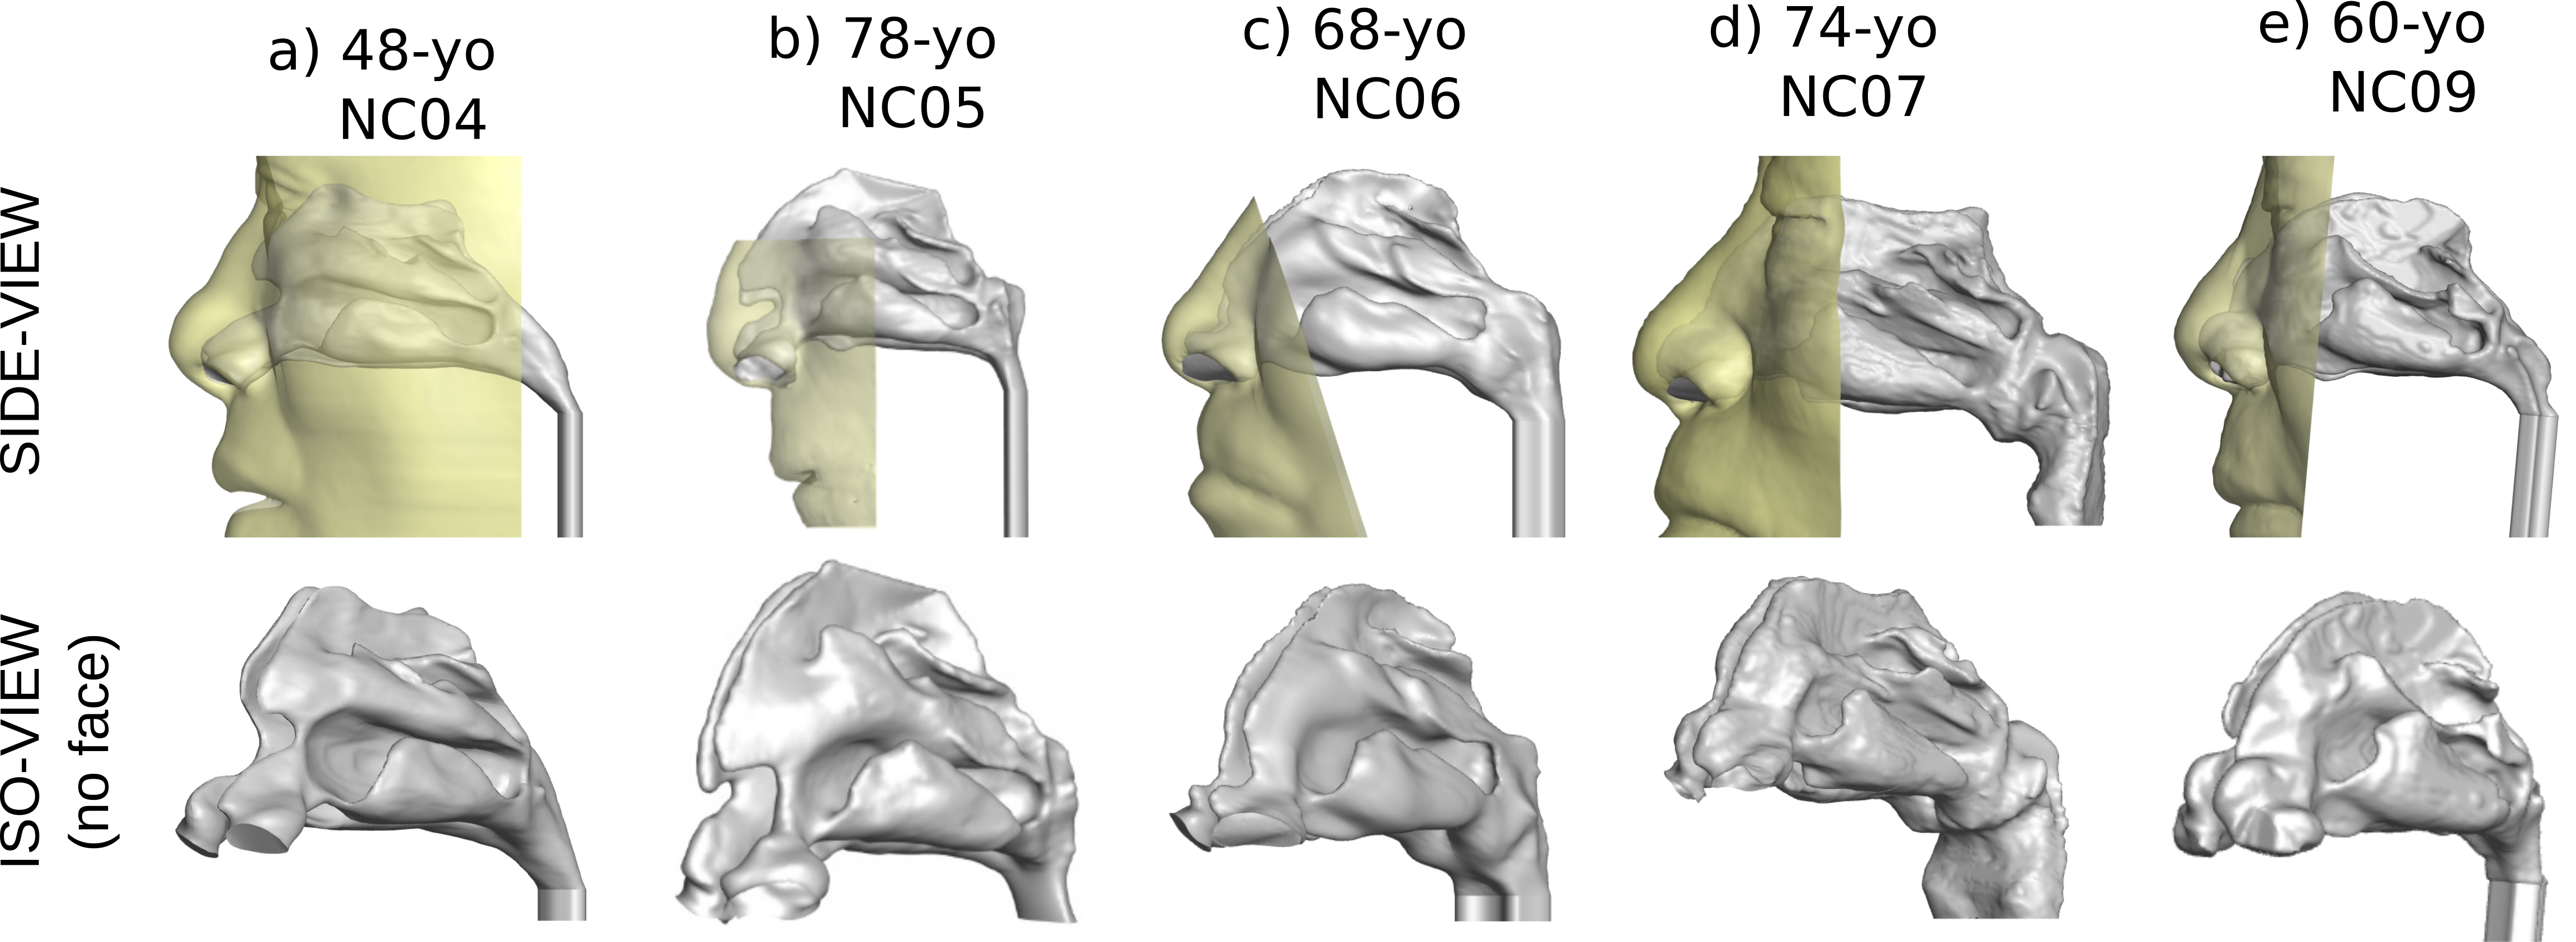
\includegraphics[width=\textwidth]{geometries}
  \caption{geometries of the five cavities}
\end{figure}

\begin{figure} 
  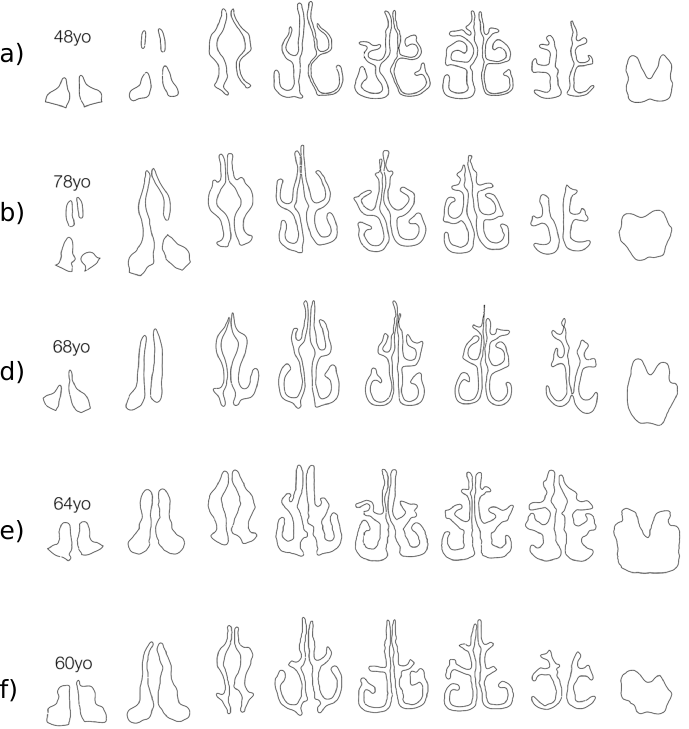
\includegraphics[width=\textwidth]{Silhouettes}
  \caption{silhouettes of the cavities}
  \label{fig:sil}

\end{figure}

\begin{figure}
  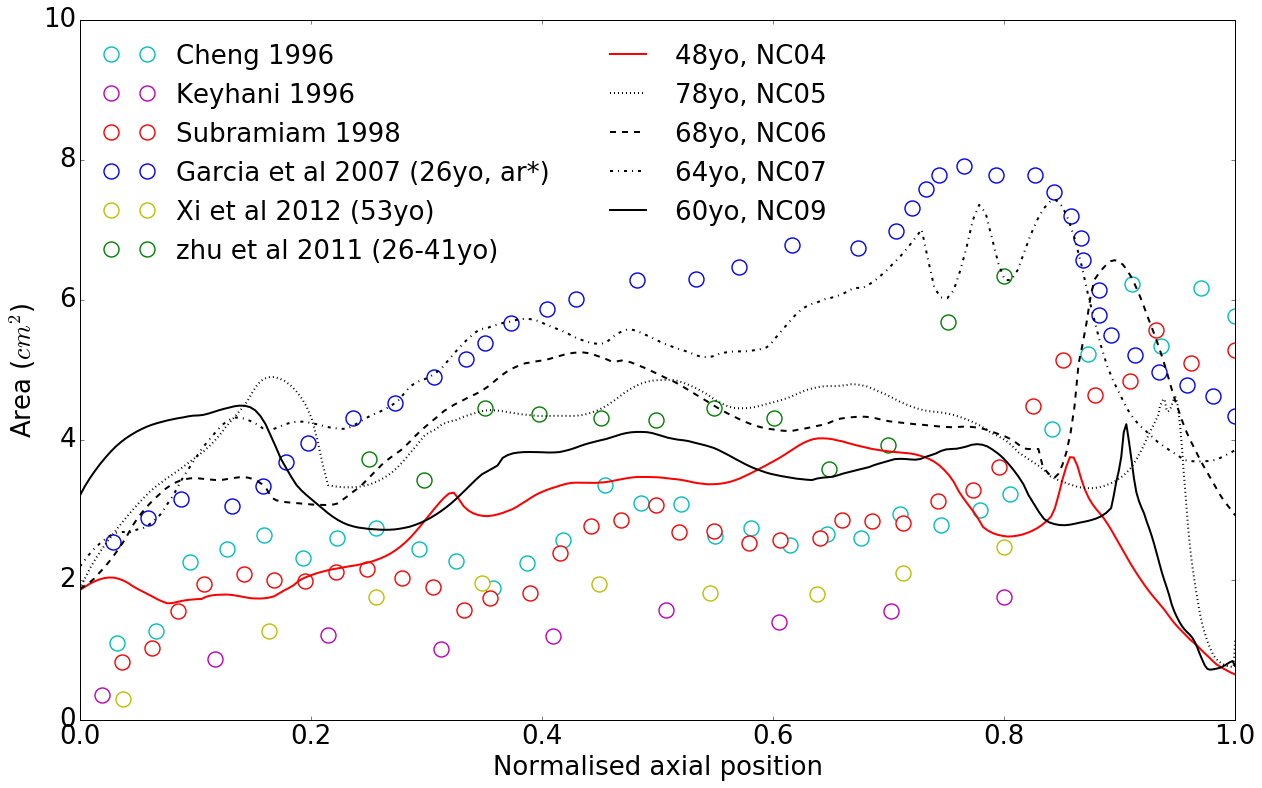
\includegraphics[width=\textwidth]{Areavsdistance}
  \caption{area versus distance across the four nasal cavities with a series of examples from the literature}
  \label{fig:area}
\end{figure}

\begin{figure}
\centering
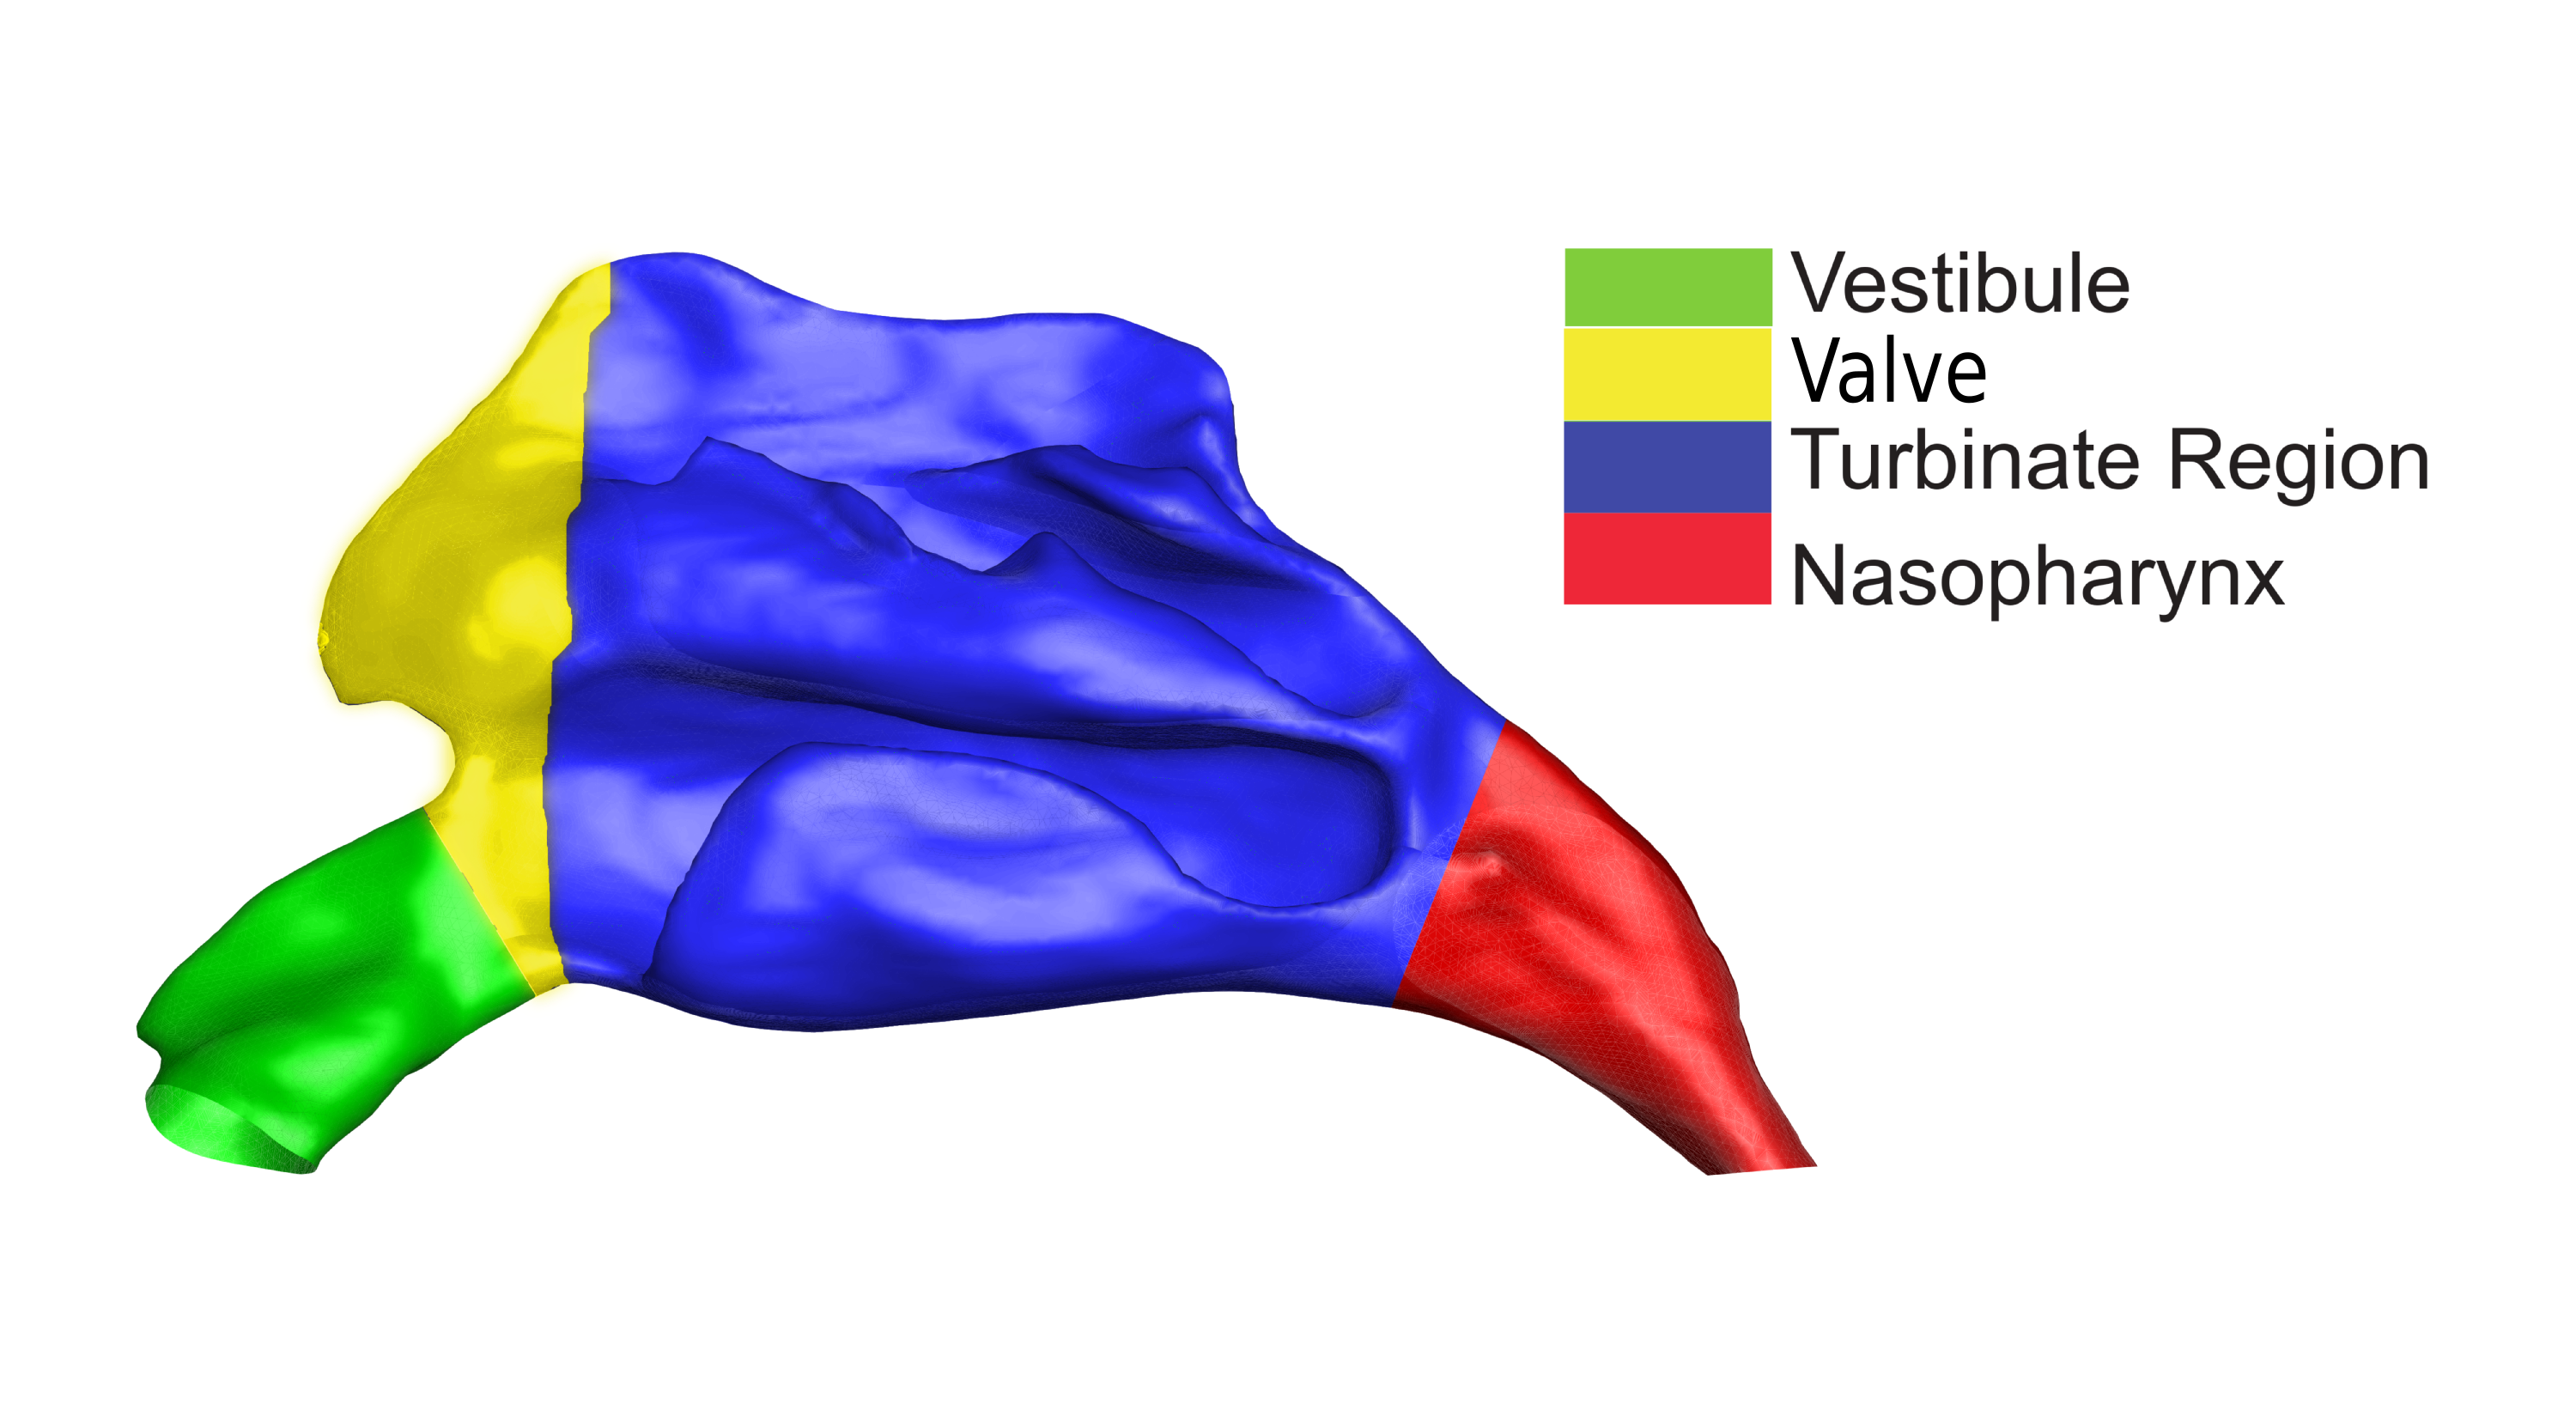
\includegraphics[width=1\textwidth]{regions}
\caption{Colour coded display of the regional divisions used in tables \ref{tab:secvol}, \ref{tab:secsa}, \ref{tab:deff}} \label{fig:regions}
\end{figure}

\begin{table}[geometric comparison]
\begin{tabular}{lllllll}
 & \textbf{NC04} & \textbf{NC05} & \textbf{NC06} & \textbf{NC07} & \textbf{Xi et al.\cite{Xi2012}} & \textbf{Garcia et al.\cite{Garcia2007}} \\
\cline{2-7}
\textbf{Turbinal region} & 18.54 & 22.78 & 24.62& 30.722& 12.63& 33.66\\
\textbf{Nasopharynx}  & 3.84 & 5.40 & 12.80 & 20.09 & 16.33 & 10.60\\
\textbf{Vestibule} & 3.10 & 4.15 & 2.81 & 4.21 & 5.50 & 2.41\\
\textbf{Total} & 25.48 & 32.33 & 40.23 & 55.07 & 34.43 & 47.77 \\
\hline
\end{tabular}
\caption{ sectional volume, according to sections as seen in Figure \ref{fig:regions} ($ cm^3 $)}\label{tab:secvol}
\begin{tabular}{lllllll}
 & \textbf{NC04} & \textbf{NC05} & \textbf{NC06} & \textbf{NC7} & \textbf{Xi et al.\cite{Xi2012}} & \textbf{Garcia et al.\cite{Garcia2007}}\\
 \cline{2-7}
\textbf{Turbinal region} & 170.92 & 174.07& 190.44 & 163.44 & 112.59 & 133.50\footnote{includes vestibule} \\
\textbf{Nasopharynx} & 12.20 & 12.80 & 25.23 & 40.42 & 40.93 & 31.46\\
\textbf{vestibule} & 15.71 & 17.37 & 12.45 & 17.92 & 35.58 &  -\\
\textbf{total} & 198.82 & 204.25 & 228.11 & 221.79 & 189.10 & 164.96\\
\hline
\end{tabular}
\caption{sectional surface area, according to sections shown in Figure \ref{fig:regions}($ cm^2 $)}\label{tab:secsa}
\begin{tabular}{lllllll}
& \textbf{NC04}  & \textbf{NC05} & \textbf{NC06} & \textbf{NC7} & \textbf{Xi et al.\cite{Xi2012}} & \textbf{Garcia et al.\cite{Garcia2007}}\\
 \cline{2-7}
\textbf{Turbinal region} & 0.434 & 0.52 & 0.52 & 0.75 & 0.45 & 1.11\\
\textbf{Nasopharynx} & 1.26 & 1.69 & 2.03 & 1.99 & 1.60 & 1.35\\
\textbf{vestibule} & 0.79 & 0.96 & 0.90 & 0.94 & 0.62 &  - \\
\textbf{total} & 0.51 & 0.63 & 0.71 & 0.99 & 0.72 & 1.13 \\
\hline
\end{tabular}
\caption{Effective diameter $d_{eff} = \frac{4v}{a} (cm) $}\label{tab:deff}
\begin{tabular}{lllllll}
\textbf{NC04}& \textbf{NC05}& \textbf{NC06}&\textbf{ NC07}& \textbf{Xi et al.\cite{Xi2012}}& \textbf{Garcia et al.\cite{Garcia2007}}\\
\hline
0.83& 1.09& 1.80& 2.29& 1.17& 2.54
\end{tabular}
\caption{Minimal axial cross sectional area $(cm^2)$}\label{tab:mca}
\end{table}

\begin{figure} 
  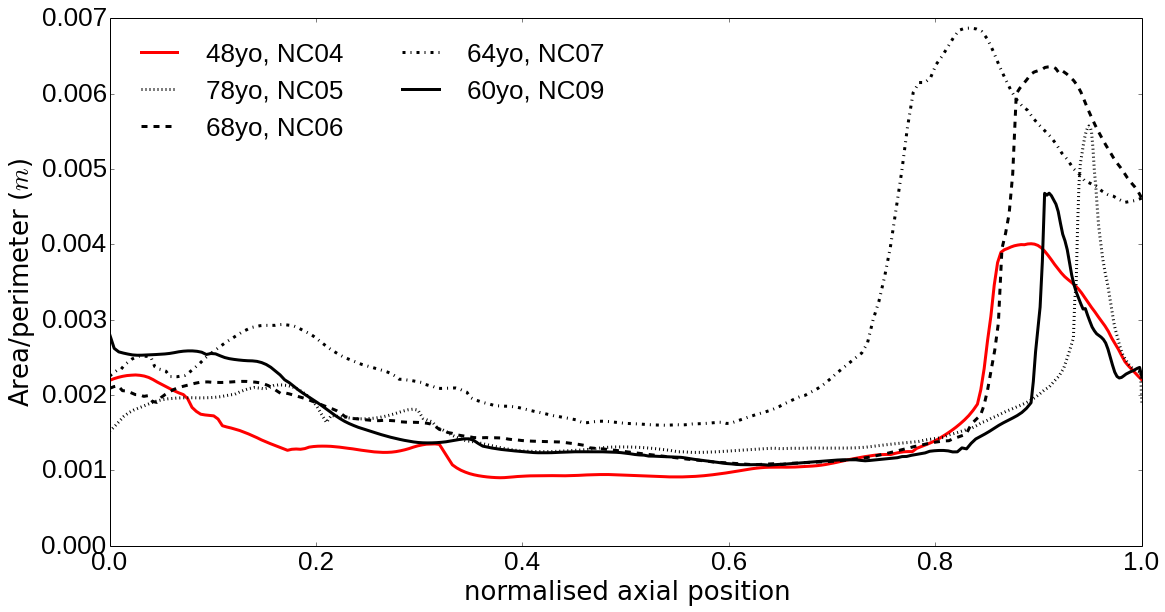
\includegraphics[width=\textwidth]{areavsperimeter}
  \caption{area versus distance across the four nasal cavities with a series of examples from the literature}
  \label{fig:arpar}
\end{figure}
\section{Pressure Drop}

The pressure drops across the nasal cavities can also be seen in Figure \ref{fig:stpr} to vary in relation to the volume of the nasal cavity. This is in contrast to the experimental findings of \cite{Lindemann2008, Edelstein1996, WhanKim2007}, who’s studies using rhinomanometry showed no significant decrease in pressure across the cavity to accompany the recorded variation in volume. The cause of this discrepancy is unclear. Here the pressure drop is primarily seen across the valve region. Here the nasopharynx has been excluded from the domain; the significant pressure drop across the nasopharynx was inversely proportional to the cross sectional areas of the respective nasal cavities

The pressure drops can be seen in Figure \ref{tab:pvv} to decrease in relation to the volume of the cavity. This fits well with the findings of previous experimental studies looking at pressure drops across nasal cavity models, as can be seen from the comparison with results from \cite{Garcia2007} and \cite{Kelly2004}, both displayed in figure \ref{tab:pvv}.

  \begin{table} 
    \centering
  \pgfplotstableset{
  every head row/.style={before row=\toprule,after row=\midrule},
  every last row/.style={after row=\bottomrule}}

  \pgfplotstabletypeset[
      fixed zerofill,
      precision=2,
      display columns/0/.style={string type},
      col sep=comma]{images/prvsflow.txt}
  \caption{Variation of pressure drop with flow rate (m/s)}
  \label{tab:pvv}
\end{table}

\begin{figure} 
  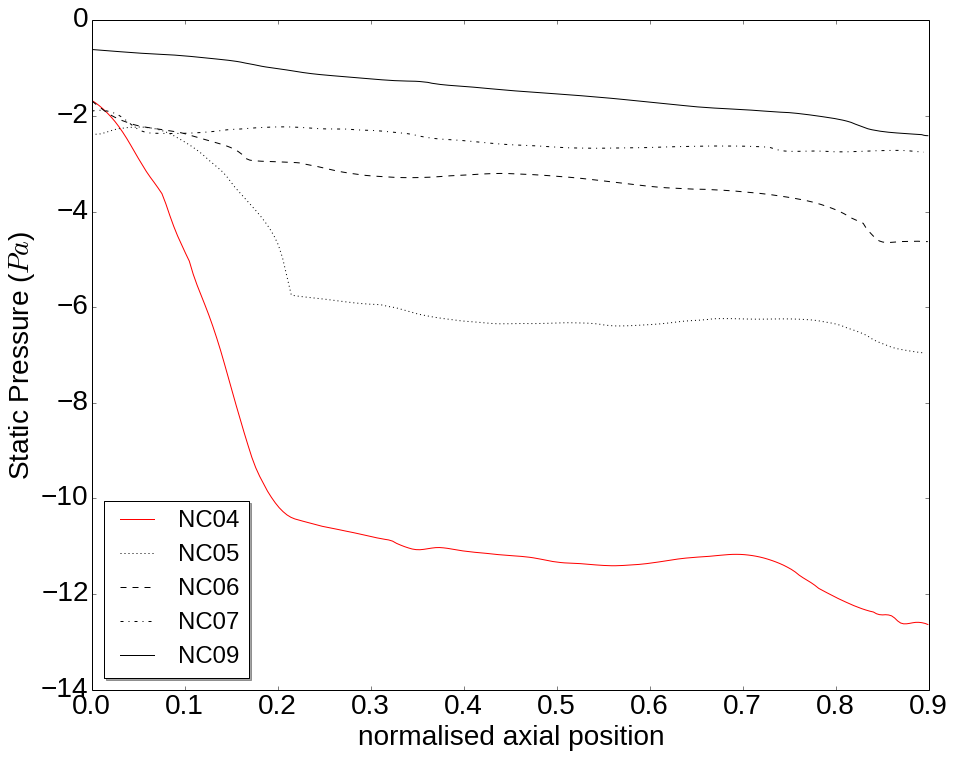
\includegraphics[width=\textwidth]{statpres}
  \caption{area versus distance across the four nasal cavities with a series of examples from the literature}
  \label{fig:stpr}
\end{figure}

\section{Wall Shear Stress}

Figure \ref{fig:wcont} shows the wall shear stress across the five models presented in this paper. The valve region can be seen to be a region of particularly high wall shear across all the models. Also note that the locations of high wall shear vary significantly in the more voluminous cavities


From Figure \ref{fig:wax}, Wall shear stress can be seen to be more pronounced in general in the more voluminous models such as NC04, and in particular this effect is exaggerated in the valve region. Here the wall shear stress is mapped rom the nostrils to the entrance to the nasopharynx. The nasopharynx showed more pronounced variations, in particular NC04 showed a significant spike in wall shear stress in the nasopharynx, which is to be expected because of its lower cross sectional area. Note that the sagittal distribution of wall shear stress is much more even in the larger cavities.  The valve region - considered of particular significance to the development of flow features within the nasal cavity \cite{Lindemann2008} – shows significant variation in wall shear stress concentration, with NC07 and NC09 presenting a very even distribution of wall shear stress, in contrast to NC04 or NC05 which show wall shear more pronounced around the opening from the vestibule. Similar variations can also be seen in the distribution within the turbinal region (Figure \ref{fig:wcont}). 

Figures \ref{fig:wcst} and \ref{fig:wcst} show the distribution of the wall shear stress around the valve and turbinate regions. The valve region - considered of particular sigtnificance to the development of flow features within the nasal cavity \cite{Lindemann2008} – shows significant variation in wall shear stress concentration, with NC07 and NC09 presenting a very even distribution of wall shear stress, in contrast to NC04 or NC05 which show wall shear more pronounced around the opening from the vestibule. Similar variations between models can also be seen in the distribution within the turbinal region. 

\begin{figure} 
  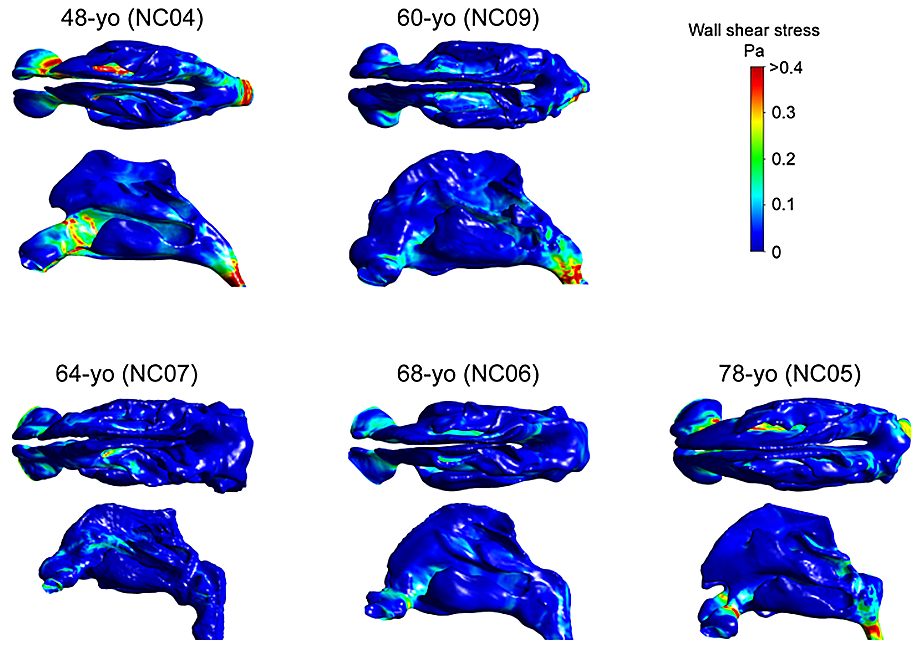
\includegraphics[width=\textwidth]{wsscont}
  \caption{isometric views of the five cavities colored by Wall shear stress}
    \label{fig:wcont}
\end{figure}

\begin{figure} 
  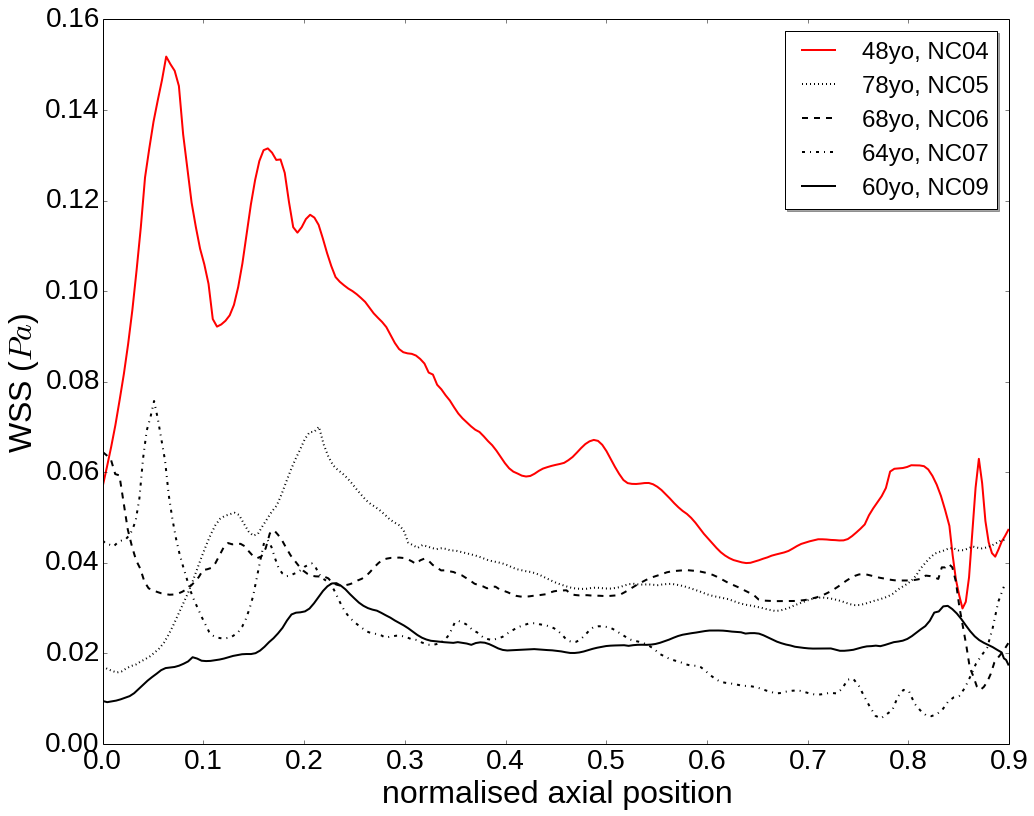
\includegraphics[width=\textwidth]{axialwss}
  \caption{coronal area weighted average of wall shear stress plotted as a function of distance from the entrance to the cavity across the saggital axis}
  \label{fig:wax}
\end{figure}

\begin{figure} 
  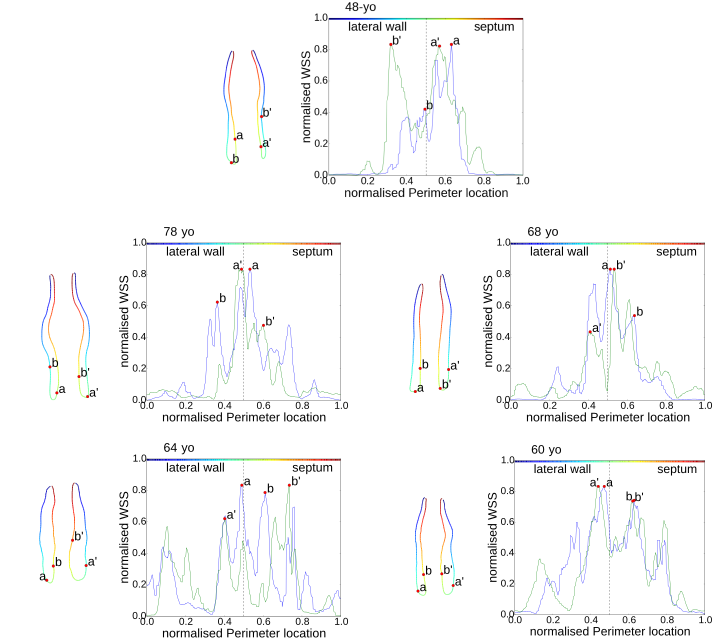
\includegraphics[width=\textwidth]{wsscsvalve}
  \caption{wall shear stress around the perimeter of the nasal valve as a function of normalised distance. See the colour scale for precise matching of graph points to location on the cavity wall. Points A and B represent the highest WSS peaks within a given cross section}
  \label{fig:wcs}
\end{figure}

\begin{figure} 
  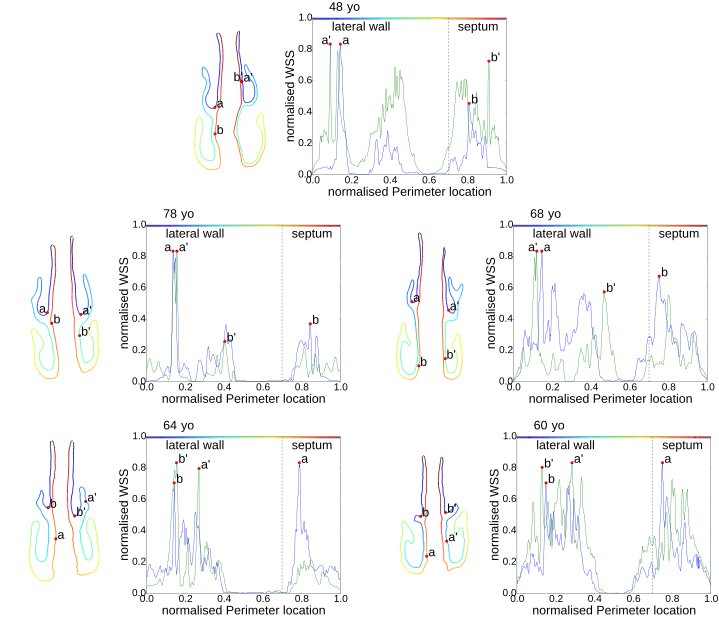
\includegraphics[width=\textwidth]{wsscsturbinal}
  \caption{wall shear stress around the perimeter of the turbinal region as a function of normalised distance. See the colour scale for precise matching of graph points to location on the cavity wall. Points A and B represent the highest WSS peaks within a given cross section}
  \label{fig:wcst}
\end{figure}

\section{Velocity}

Some discrepancies can be observed in the airflow contours between the models of different capacities in Figure \ref{fig:vcc}. Note the more even distribution of sagittal airflow in the more voluminous models, particularly notable in NC07 and NC09, when compared with the narrower cavities such as NC04 or NC05. This is particularly prominent in the valve and Turbinal regions. The increasing vorticity seen across the models of increasing volume – particularly in the valve region – is epitomised in the atrophic rhinitis model from Garcia et al\cite{Garcia2007}.

The streamlines show a reduced linearity to the flow as the cavities increase in volume; this is particularly evident in the valve and nasopharynx reasons. This varies somewhat from the atrophic rhinitis model, where the most prominent turbulence is in the lower meatus. This is probably related to the significant degeneration seen in the turbinal region of the rhinitis model.

\begin{figure} 
  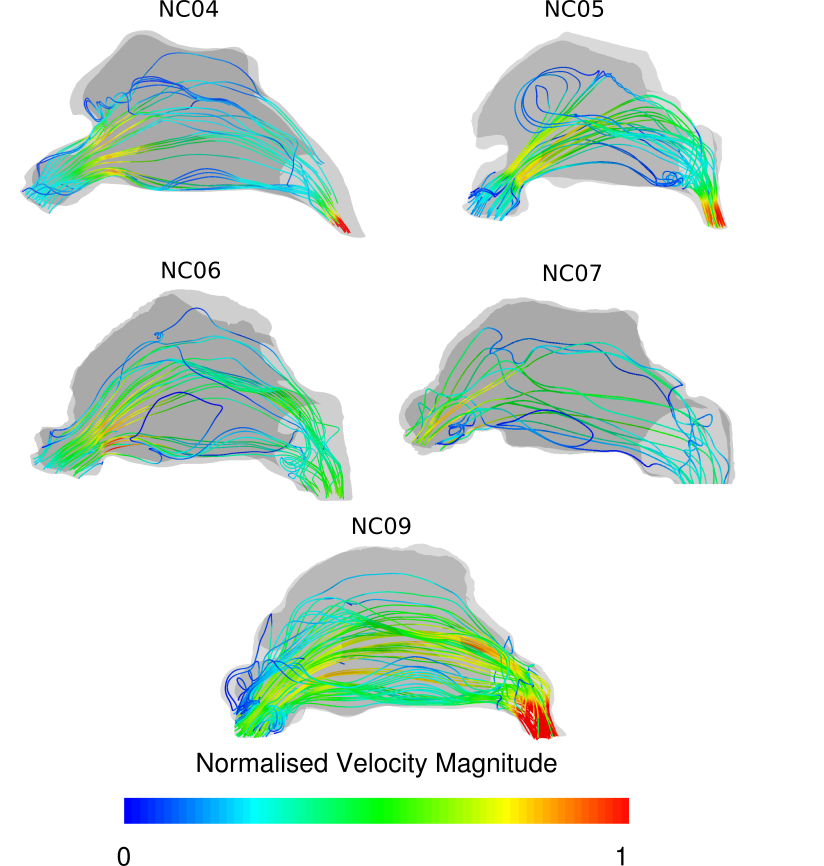
\includegraphics[width=\textwidth]{streamlines}
  \caption{streamlines seeded uniformly across the entrance to the nasal cavity, coloured by velocity magnitude, normalised across for the range of each cavity}
  \label{fig:vsl}
\end{figure}

\begin{figure} 
  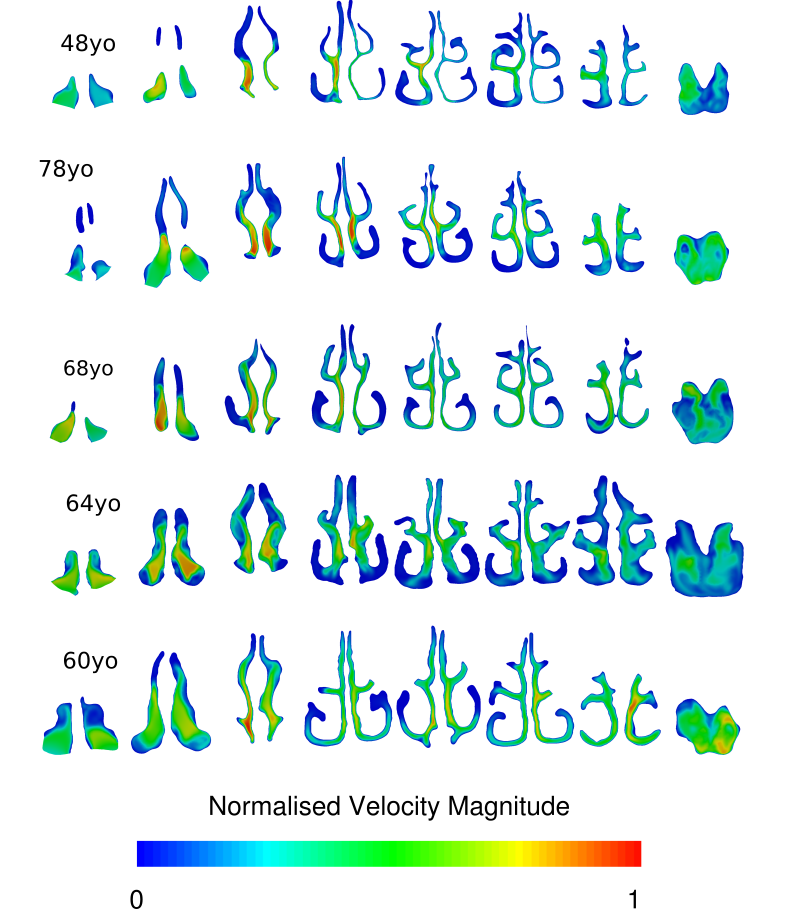
\includegraphics[width=\textwidth]{coroconts}
  \caption{Coronal cross sections, taken at 8 equidistant locations across the sagittal axis, coloured by normalised velocity magnitude}
  \label{fig:vcc}
\end{figure}

\section{Heat and Vapour Transfer}
